\section{Rozdział Paweł Czernecki}

Wyrażenie matematyczne:
\[e^{i\pi}+1=0\]


Zdjęcie:
\begin{figure}[h!]
  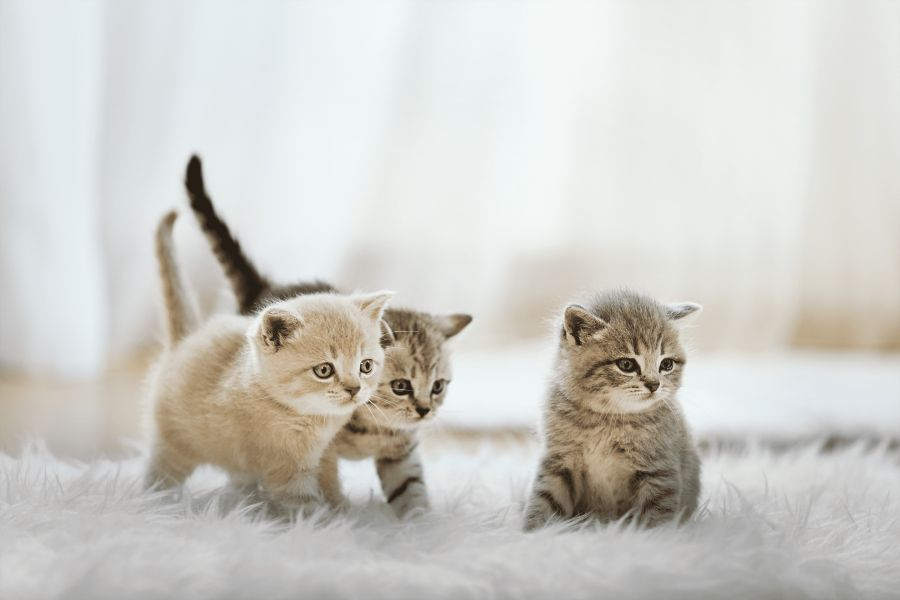
\includegraphics[width=7cm]{pictures/1648545312.jpg}
  \caption{Kotki}
  \label{fig:cats}
\end{figure}


Tabela:\newline
\begin{tabular}{lllll}
lp & nazwa    & cena &  \\
1. & produkt1 & 12   &  \\
2. & produkt2 & 13   &  \\
\end{tabular}



Lista numerowana:
\begin{enumerate}
    \item Item1
    \item Item2
    \item Item3
\end{enumerate}


Lista nienumerowana:
\begin{itemize}
  \item[-] Item1
  \item[-] Item2
  \item[-] Item3
\end{itemize}

\textbf{Pierwszy paragraf} of a section which, as you can see, is not indented. This is more text in the paragraph. This is more \textit{text} in the paragraph.

\textbf{Drugi paragraf} of a section which, \underline{as you can see, is not indented.} This is more text in the paragraph. This is more text in the paragraph. Zawierający odwołanie do rysunku: \ref{fig:cats}